\documentclass{matmex-diploma-custom}



\begin{document}
% Год, город, название университета и факультета предопределены,
% но можно и поменять.
% Если англоязычная титульная страница не нужна, то ее можно просто удалить.
\filltitle{ru}{
 university = {Правительство Российской Федерации\\Федеральное государственное бюджетное образовательное учреждение высшего профессионального образования\\
«Санкт-Петербургский государственный университет»},
	faculty = {\hfill},
    chair              = {Кафедра Системного Программирования},
    title              = {Скрытые Марковские модели переменного порядка для анализа
данных ChIP-seq},
    % Здесь указывается тип работы. Возможные значения:
    %   coursework - Курсовая работа
    %   diploma - Диплом специалиста
    %   master - Диплом магистра
    %   bachelor - Диплом бакалавра
    type               = {bachelor},
    position           = {студента},
    group              = 444,
    author             = {Атаманова Анна Михайловна},
    supervisorPosition = {д.\,ф.-м.\,н., профессор},
    supervisor         = {Терехов А.\,Н.},
    reviewerPosition   = {},
    reviewer           = {},
    chairHeadPosition  = {д.\,ф.-м.\,н., профессор},
    chairHead          = {Терехов А.\,Н.},
%   university         = {Санкт-Петербургский Государственный Университет},
%   faculty            = {Математико-механический факультет},
%    city               = {Санкт-Петербург},
%   year               = {2015}
}
\filltitle{en}{
	type 			  = {bachelor},
	faculty 			  = {\hfill},
    chair              = {Chair of Software Engineering},
    title              = {Variable-length hidden Markov models for ChIP-seq data analysis},
    author             = {Anna Atamanova},
    supervisorPosition = {professor},
    supervisor         = {Andrey Terekhov},
    reviewerPosition   = {},
    reviewer           = {},
    chairHeadPosition  = {professor},
    chairHead          = {Andrey Terekhov},
}
\maketitle
\tableofcontents
% У введения нет номера главы
\section*{Введение}
\subsection*{Предметная область}
Наш организм есть огромное множество клеток. Клетки постоянно движутся, строят, разрушают. Вся жизнь наша заключается в их функционировании. Одна из интереснейших частей клетки --- это ее память, ДНК (дезоксирибонуклеиновая кислота), которая хранит в себе просто неимоверное количество информации, в том числе <<рецепты>> построения необходимых веществ. Своеобразным строительным материалом клетки является белок. Белок также выполняет структурные, сигнальные, механические и другие функции. Соединения ДНК с конкретным белком могут играть роль в структуре клетки, во внутренних механизмах ее управления. Поэтому изучение ДНК-белковых взаимодействий крайне важно и актуально.

Однако перед самим изучением взаимодействий, необходимо обнаружить/распознать места, где они случились.

Данная работа посвящена изучению нахождения позиций связывания конкретного белка и ДНК, то есть нахождения позиций ДНК-белковых взаимодействий при заранее выбранном белке.

\subsection*{ChIP-seq}
ChIP-seq (chromatin immunoprecipitation sequencing) --- биологический эксперимент, который по тысячам одинаковых клеток и выбранному белку, выдает вектор длины генома из 0 и 1, где 1 обозначает, что в окрестностях данной позиции ДНК был замечен белок, 0 - обратное.

Более подробно, но по-прежнему глубоко утрировано, все происходит следующим образом. Сначала, в клетки заливается специальный раствор, который приклеивает белки к ДНК. Потом, с помощью ультразвука, ДНК разрезаются на более мелкие фрагменты. Далее специальным антителом, подобранным к данному белку, вылавливаются те фрагменты, которые были связаны с исследуемым белком. Затем специальный прибор -- секвенатор считывает концы фрагментов (целый фрагмент слишком велик для считывания). Считанный кусок фрагмента называется прочтением или ридом. 
Так продолжается, пока каждый фрагмент не будет с высокой вероятностью считан несколько раз.

Далее для каждого полученного рида ищется соответствующий
ему участок последовательности генома (рис.~\ref{fig:chip-seq}). Обычно
риды, которым может соответствовать более одного участка в геноме,
исключают из рассмотрения.

\begin{figure}[h]
  \centering

\begin{Verbatim}[commandchars=\\\{\}]
          CAAAAGACAAATAGTGATGTCACCAATCGAGC
          --------------------------------
               GACA ATA     GTCA  AATC
              AGAC   TAGTG TGTC
               GACA   AGTG TGTCA   ATCG

          00001100001110000110000011000000
\end{Verbatim}
  \caption{Схематическое изображение выравнивания прочтений секвенатора (под чертой)
    на известную последовательность генома (над чертой).}
  \label{fig:chip-seq}
\end{figure}

Результаты эксперимента представляют в виде вектора длины генома, в котором
стоит 1, если в соответствующей позиции генома начиналось хотя бы одно прочтение
и 0 в обратном случае.

Однако белок мог находиться не в самом начале фрагмента, и, кроме того, соединение белка с ДНК происходит не точечно, а на некотором участке ДНК.
По этому, для дальнейшего анализа, полученный вектор разбивается на отрезки заранее выбранной длины, называемые окнами (обычно 200 пн (пар нуклеотидов)). Значение в окне определяется, как сумма единичек в нем. 

Эксперимент ChIP-seq (как и большинство биологических
экспериментов) не исключает наличие ошибок в результатах. Недостаточная специфичность антитела, наличие ошибок секвенирования, нестабильность положения белка на ДНК приводят к возникновению сигнала не
зависящего от наличия взаимосвязи.
По этому, для дальнейшего анализа результатов эксперимента, требуется построение некоторой вероятностной модели, способной отделять ошибки, а также 
выявлять зависимости соединений и, по возможности, описывать их структуру.
Большинство существующих моделей (\cite{Zhang2008}, \cite{Spyrou2009}) для данных
хроматин-иммунопреципитации основано на аппарате скрытых Марковских моделей (СММ) \cite{Rabiner1989}
первого порядка с Пуассоновскими испусканиями. Использование распределения
Пуассона для покрытия опирается на предположение о том, что в каждой
позиции генома в среднем начинается одинаковое количество прочтений.
Марковский процесс, как правило, имеет два состояния <<$+$>> --- сигнал есть и <<$-$>> --- сигнала нет. Первой порядок модели означает, что состояние некоторого окна зависит только от состояния его прямого предшественника.
Использование моделей первого порядка объясняется тем, что количество параметров
модели, а также сложность её обучения и использования экспоненциально зависят от
порядка. Так СММ порядка $ m $ для каждой цепочки из $ m $ состояний содержит распределение на следующее состояние ($ 2^m $ вероятностных распределений). В связи с этим неправильный выбор $ m $ в обучении сильно усложняет модель и способствует ее переобучению. 

Скрытые Марковские модели переменного порядка избегают такой эффект, т.к. они не фиксируют длину строки порождающей следующее состояние и стараются ее уменьшить.

\section{Постановка задачи}
Цель данной дипломной работы --- построение скрытой Марковской модели переменного
порядка для анализа данных ChIP-seq.

Для достижения цели были определены следующие задачи.
\begin{enumerate}
\item
Реализация скрытой Марковской модели
переменного порядка.
\item
Анализ эффективности работы модели на синтетических
данных, сравнение с более простыми моделями (СММ
первого порядка)
\item
Применение к данным ChIP-seq.
\end{enumerate}


\section{Обзор существующих решений}
Марковские модели переменного порядка (не скрытые) обучаются путем построения контекстного дерева переходов \cite{Buhlmann1999}. Скрытые Марковские модели фиксированного порядка обучаемы алгоритмом Баума-Велша \cite{Rabiner1989}.
Совмещение этих двух идей дает возможность обучить скрытые Марковские модели переменного порядка (СММПП). Такой подход обучения был предложен в \cite{Wang2006}. 

Итоговым алгоритмом обучения СММПП был выбран слегка модифицированный под поставленную задачу алгоритм  из \cite{Wang2006}, дополненный недостающей информацией об обучении контекстных деревьев из статей \cite{Buhlmann1999}, \cite{Dumont2014}.

Модификация заключается в следующем: наблюдения итоговой модели будут порождаться не из контекстов, а из соответствующих состояний, т.е. распределение значений для каждого окна будет задаваться скрытым состоянием, которое определяет, была ли там взаимосвязь с белком или нет. 

\subsection{Основные понятия и определения}

Путь 
$ S = \{0, 1\} $ --- множество состояний (в нашем случае 1 будет обозначать связь, 0 -- обратное), 
$X_0, X_1, \ldots $ --- последовательность случайных величин (дискретный случайный процесс), значения которых лежат в S, 
$x_0, x_1, \ldots$ - некоторая реализация случайных величин $X_0, X_1, \ldots $.

\begin{definition} $ \{X_{i}\}_{i \in Z_{+}}$ называется \emph{Марковским процессом порядка $ m $}, если  
\begin{align*}
&\forall t, t'\in N, \;t, t' \geq m,\; \forall x_{t},x_{t-1},\ldots ,x_{0}\in S
\\&P(X_{t} = x_{t}|X_{t-1}=x_{t-1},X_{t-2}=x_{t-2}, \ldots ,X_{0}=x_{0}) 
\\&=P(X_{t} = x_{t}|X_{t-1}=x_{t-1},X_{t-2}=x_{t-2}, \ldots ,X_{t-m}=x_{t-m})
\\&=P(X_{t'} = x_{t}|X_{t'-1}=x_{t-1},X_{t'-2}=x_{t-2}, \ldots ,X_{t'-m}=x_{t-m})
\\&=P(X_{t'} = x_{t}|X_{t'-1}=x_{t-1},X_{t'-2}=x_{t-2}, \ldots ,X_{0}=x_{0}) 
\end{align*}
\label{MP}
\end{definition}
Далее, имея дело с Марковским процессом, вероятности вида  
$$P(X_{t'} = x_{t}|X_{t'-1}=x_{t-1},X_{t'-2}=x_{t-2}, \ldots ,X_{t'-m}=x_{t-m})$$ где $t'\geq m$, будем записывать как $P(x_{t} |x_{t-1}\ldots x_{t-m})$ (запись корректна, в силу независимости такой вероятности от $t'$).

Для удобства будем считать, что наш процесс растет справа налево  
$$\ldots x_{t},~ x_{t-1},~ x_{t-2} \ldots$$
Так,  если цепь $\ldots x_{t}, x_{t-1}, x_{t-2} \ldots$ была порождена процессом порядка $2$,
то $$P(x_{t}| x_{t-1},x_{t-2}\ldots) = P(x_{t}|x_{t-1},x_{t-2})$$

\begin{definition} \emph{Марковская модель порядка $ m $} --- это вероятностная модель, описывающая марковский процесс порядка $m$. Параметрами модели являются множество переходов  $ A = \{a(q; x^{m})\}_{q \in S, x^{m} \in S^{m}}$, где $a(q; x^{m}) = P(q|x^{m})$, и начальное распределение $\pi = \pi(x^m)_{x^m \in S^m}$, где $\pi(x^m) = P(X_{0:m}=x^m)$.
\end{definition}

Другими словами, \textit{Марковский процесс порядка $m$} --- это случайный процесс, текущее состояние которого зависит лишь от $m$ предшествующих состояний и не зависит от времени. Таким образом, любая строка из $m$ состояний задает распределение на следующее за ней состояние. 

\textit{Контекстом} состояния $ x_{t} $  называется любой префикс строки  $x_{t-1}, x_{t-2} \ldots$. 

\begin{definition}
\textit{Контекстное дерево} --- дерево, в котором каждая внутренняя вершина имеет $ |S| $ ребер соответствующих состояниям из $S$ и метку, которая является конкатенацией метки на ее родителе и метки ребра от него. Метка в корне - пустая строка.
\end{definition}
Теперь множество переходов для Марковского процесса порядка $ m $ можно определить как контекстное дерево глубины $ m+1 $, каждый лист которого содержит распределение $P(.~|~w)$, где $ w $ --- метка на листе.

Для того, чтобы по дереву определить распределение следующего состояния $ x_{t} $, достаточно из корня спуститься по ветке, вершины которой соответствуют контекстам этого состояния, $(x_{t-1}),\; (x_{t-1}x_{t-2}), \ldots$ . Лист на конце ветке будет задавать распределение состояния $ X_{t} $.

Контексты, соответствующие листьям контекстного дерева будем называть \textit{главными контекстами} (иногда, когда речь будет идти только о листьях, слово <<главные>> будем опускать).

\begin{remark}
Пометки на листьях контекстного дерева определяют все дерево.
\end{remark}

На рисунке \ref{ris:context_trie} изображен пример контекстного дерева переходов для Марковского процесса порядка $ 2 $ (серым подкрашены листья, ниже прямоугольниками обозначены распределения переходов).
\begin{figure}[h!]\centering
\begin{minipage}[b]{0.49 \textwidth}
	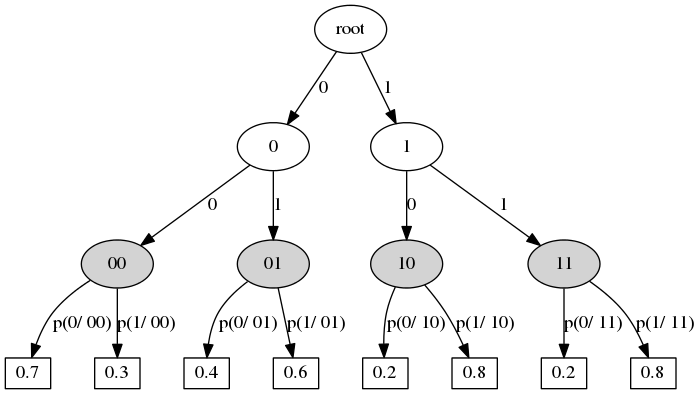
\includegraphics[scale=0.38]{img/Context_trie.pdf}
	\centering
	\caption{ Контекстное дерево переходов Марковского процесса порядка 2 }
	\label{ris:context_trie}
	
\end{minipage}
\hfil \hfil
\begin{minipage}[b]{0.49 \textwidth}
	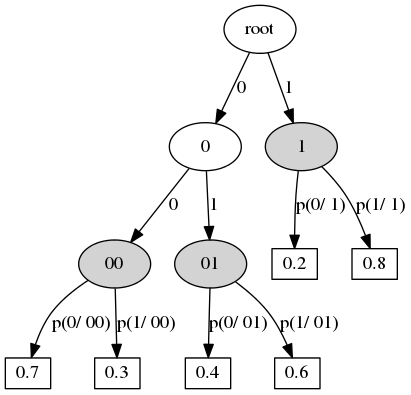
\includegraphics[scale=0.4]{img/Prune_c_trie.png}
	\centering
	\caption{ Подрезанное контекстое дерево }
	\label{ris:prune_c_trie}
\end{minipage}
\end{figure}
Можно заметить, что в этом примере, имея для некоторого состояния $x_{t}$ контекст  <<$1$>> , необходимость уточнять его (т.е. спускаться дальше к листу) отсутствует, т.к. распределение на контекстах  <<$10$>>  и  <<$11$>>  одно и тоже. 
Таким образом подстриженное дерево с рисунка \ref{ris:prune_c_trie} задает такие же распределения переходов как и дерево с рисунка \ref{ris:context_trie}. 
Однако второе контекстное дерево меньше (число главных контекстов меньше).
Но не один Марковский процесс фиксированного порядка напрямую его использовать не может.
Определим процесс, который может иметь распределение переходов в виде такого дерева.

Пусть $\tau$ --- конечное контекстное дерево.
Для $s \in \tau$ будем обозначать через $ C(s) $ множество всех потомков, являющихся листами $\tau$. 
Для $s \notin \tau$, $C(s)$ --- лист $\tau$, являющийся префиксом  $s$ (можно заметить, что он существует и единственен)
\begin{definition}
\textit{Марковский процесс переменного порядка} с максимально-возможным порядком $m$ --- это вероятностный процесс, распределения на состояниях которого задаются распределниями на листьях некоторого контекстное дерево $\tau$ глубины не более, чем $m+1$, и 
\[ P(q |s) =
  \begin{cases}
    P(q|C(s))       & \quad \text{для} s \notin \tau\\
    \frac{\sum_{c \in C(s)} {P(q|c)p(c)}}{\sum_{q' \in S}\sum_{c \in C(s)} {P(q'|c)P(c)}} & \quad \text{для} s \in \tau\\
  \end{cases}
\]
вероятность того, что следующее состояние за цепью $s$ является $q$
\label{def:c_trie}
\end{definition}

\begin{definition}
Марковская модель переменного порядка с максимально-возможным порядком $m$ --- вероятностная модель, описывающая соответствующий процесс.
Параметрами модели являются множество переходов на листьях некоторого контекстного дерева $\tau$ глубины не более чем $m+1$ и вероятностное распределение на них (листьях).
\end{definition}

\begin{remark}
ММПП с максимально-возможным порядком $m$ есть обобщение всех скрытых Марковских процессов порядка меньше либо равного, чем $ m $.
\end{remark}

\subsection{Скрытые Марковские модели}
Представим, что состояния -- это какой-то скрытый признак/фактор (например, наличие или отсутствие связи белка и ДНК) цепи наблюдений $Y = \{y_{t}\}_{t \in Z_{+}}$. Для каждого наблюдения $y_{t}$ он не известен, однако он его определяет.


Тогда, имея Марковскую цепь $X = \{x_{t}\}_{t \in Z_{+}}$ и покоординатно определяя для каждого состояния $x_{t}$ новую случайную величину $Y_{t}$ согласно распределению $P(.|~x_{t})$, можно задать цепь
$Y = \{y_{t}\}_{t \in Z_{+}}$ .

\begin{definition}
Процесс, порождающий цепь по некоторой Марковскому процессу $X = \{x_{t}\}_{t \in Z_{+}}$ порядка $m$ и распределению $P(.|~x_{t})$, называется \textit{скрытым Марковским процессом порядка $m$}. 
$ X $ называеются \textit{скрытыми состоянияниями}, $Y$ --- \textit{наблюдениями}.
\end{definition}

\begin{definition}
\textit{скрытая Марковска модель} (СММ) порядка $ m $ --- вероятностная модель, описывающая соответствующий процесс. Параметрами модели является $\Lambda=(A,\pi,B)$, где $A,\pi$ --- параметры скрытого процесса $X$ порядка $m$,  $ B = \{b(y,x)\}_{y \in R^{l}, x \in S}$, где $ b(y; x) = P(y|x)$ ---  множество распределений испусканий. 
\end{definition}

\begin{definition}
\textit{скрытая Марковска модель переменного порядка} (СММПП) --- вероятностная модель, описывающая соответствующий процесс. Параметрами модели является $\Lambda=(A,\pi,B)$, где $A,\pi$ --- параметры скрытого процесса переменного порядка $X$ ,  $ B = \{b(y,x)\}_{y \in R^{l}, x \in S}$, где $ b(y; x) = P(y|x)$ ---  множество распределений испусканий. 
\end{definition}


\subsection{Обучение модели СММПП}
{\large Задача:} 
\\
По цепи наблюдений $ Y = (y_{1}, ... y_{T}) $ найти параметры $\Lambda = (A,B,C,\pi)$ модели СММПП, которые бы максимизировали правдоподобие модели, минимизируя при этом длины контекстов. При этом, параметр алгоритма $ \epsilon_{\text{prune}} $ будет определять допустимое отклонение распределений, которым можно жертвовать в пользу уменьшения числа контекстов.
%Другими словами, найти
%\begin{align*}
%\Lambda = \arg\!\min_{\Lambda}{\{|\Lambda(C)|\;|\Lambda \in \arg\!\max_{\Lambda}%{\{P(Y|\Lambda)\}}\}}
%\end{align*}
\\\\
{\large Алгоритм:}
\\
Параметры алгоритма: 
$ m $ --- максимальная длина контекста, 
$ \epsilon_{\textit{EM}} $ --- порог для остановки EM,
$ \epsilon_{\textit{prune}} $ --- порог для обрезания дерева
\\
\begin{enumerate}
\item Инициализация контекстов.
$$ C = S^{m}$$
множество из всех строк длины $m$.
\\
Начальные распределения переходов произвольные.
В определенных случаях (Gauss, Poisson) частотное распределение, полученное из цепи алгоритмом k-means (k=m), ускоряет работу
\\
\item EM (Expectation–Maximization algorithm).
\\
Пересчет производится подобно алгоритму Баума-Велша для СММ \cite{Rabiner1989}.
\\
\begin{enumerate}
\item E-шаг (Expectation)\\
Вводятся дополнительные параметры:
$$ \alpha_{t}(c) = P(y_{0}^{t}, c(x_{t})=c| \Lambda)$$
вероятность породить первые $t+1$ наблюдений равными $y_{0}^{t}$, имея главным контекстом  скрытого состояния $x_{t}$ контекст $ c $, из модели СММПП с параметрами $\Lambda$
\\
$$ \beta_{t}(c) = P(y_{t+1}^{T}| c(x_{t})=c, \Lambda))$$
вероятность того, что последние $T-t$ наблюдений цепи длины $T$, порожденной из модели СММПП с параметрами $\Lambda$, в которой главный контекст скрытого состояния $x_{t}$ является $ c $, совпадают с $y_{t+1}^{T}$
\\
$$ \gamma_{t}(c) = P(x_{t}=c|Y,\Lambda) $$ 
вероятность того, что породив цепь $Y$ моделью СММПП c параметрами $\Lambda$,
главный контекст скрытого состояния $ x_{t} $ является $c$. 

Зная параметры модели, нововведенные параметры считаются следующим образом:
\begin{center}
$$ \alpha_{0}(c) = \pi(c)b(y_{0},c)$$ 
$$ \alpha_{t+1}(c) = \sum_{q \in S, c'=C(cq)}{\alpha_{t}(c')a(c[0];c')b(y_{t+1},c[0])}$$
\\
$$ \beta_{T}(c) = 1$$ 
$$ \beta_{t}(c) = \sum_{q \in S, c'=C(qc)}{a(q;c)b(y_{t+1}, c'[0])\beta_{t+1}(c')}$$
$$p = P(Y|\Lambda) = \sum_{c \in C}\alpha_{T}(c)$$
правдоподобие модели
\\ 
$$ \gamma_{t}(c) = \frac{\alpha_{t}(c)\beta_{t}(c)}{p}$$
\end{center}
\item M-шаг (Maximization)\\
На этом шаге, алгоритм обновляет параметры модели максимизируя правдоподобие, при условии посчитанных $\alpha, \beta, \gamma$;

Для пересчета множества распределений переходов вводится еще один дополнительный параметр $\xi$
\begin{align*}
\xi_{t}(q;c) = P(c(x_{t})=c, x_{t+1} = q| Y, \Lambda)
\end{align*}
вероятность того, что породив цепь $Y$ моделью СММПП c параметрами $\Lambda$, 
главный контекст скрытого состояния $ x_{t} $ является $c$ и состояние $ x_{t+1} $ совпадает с $q$
\begin{align*}
\xi_{t}(q;c) = \frac{\alpha_{t}(c)a(q;c)b(y_{t+1},q)\beta_{t+1}(qc)}{p} 
\end{align*}
Обновление $ A $ по $ \xi $\\
$$ a(q; c) = \frac{\sum_{t}\xi_{t}(q,c)}{p(c)}$$
Обновление $\pi$
$$\pi(c) = \sum_{t}\gamma_{t}(c)$$

Пересчет $ B $ зависит от принятого семейства моделей испусканий и производится с помощью $ \gamma $ в точности также как и в алгоритме Баума-Велша.
В случае распределения Пуассона
$b(.~|~c) \sim Poisson(\lambda_{c})$ 
пересчет параметров происходит следующим образом
$$ \lambda_{c} = \frac{\sum_{t}{\gamma_{t}(c)y_{t}}}{\sum_{t}{\gamma_{t}(c)}}$$
\end{enumerate}
EM-алгоритм запускает поочередно E-шаг и M-шаг, пока правдоподобие с предыдущей итерации отстает от правдоподобия с текущей итерации более, чем на $ \epsilon_{\textit{EM}}$
(т.е. пока итерация дает значимый прирост правдоподобия)
\item Обрезание дерева.\\
Если существует внутренний лист контекстного дерева $ s $ такой, что 
$$ \forall q \in S \; P(sq)kl(sq, s) < \epsilon_{\textit{prune}} $$
(дети не уточняют родителя), то $ s $ становится листом, а все его потомки обрезаются, где
\begin{align*}
kl(u, w) = \sum_{q' \in S} P(q'|u) log\frac{P(q'|u)}{P(q'|w)}
\end{align*}
расстояния Кульбака-Лейблера для апостериорных распределений.
Если таких листьев не существует, алгоритм заканчивает работу.
\item Пересчет параметров $ A $, $\pi$ на новых контекстах.
$$a_{\textit{new}}(q; c_{\textit{new}}) = P(q| c_{\textit{new}})$$
пересчитывается по определению [\ref{def:c_trie}] контекстного дерева
\begin{align*}
\pi_{\textit{new}}(c_{\textit{new}}) = \sum_{c \in C(c_{\textit{new}})}{\pi(c)}
\end{align*}
$$
a = a_{\textit{new}},\;\;
\pi = \pi_{\textit{new}}
$$
Переход на второй шаг (EM-алгоритм).

\end{enumerate}

\begin{remark} При пересчете вероятности могут очень близко подходить к нулю, что отрицательно влияет на точность расчета. Для избежания этой проблемы все расчеты следует проводить не с вероятностями, а с их логарифмами.
\end{remark}
\begin{remark} EM следует запускать несколько раз, т.к. он может застревать в локальных максимумах функции правдоподобия.
\end{remark}

\subsection{Обучение на нескольких выборках}
В случае пропусков или разрывов в наблюдениях (связанных, например, с отсутствием данных), обучение модели может проходить на множестве из нескольких цельных кусков.
\\
Т.е. на вход алгоритма будет подаваться не одна выборка $Y$, а                                                                                                                                                                                                                                                                                                                                                                                                                                                                                                                                                                                                                                                              $ N $ выборок $ \{Y^{1} \ldots Y^{N}\}$ подчиненных единому скрытому Марковском процессу переменного порядка.
\\
Приведем небольшие корректировки алгоритма выше для решения этой задачи.
\\
EM-алгоритм
\begin{enumerate}
\item Expectation\\
Дополнительные параметры $\alpha^{d}, \beta^{d}, \gamma^{d}, \xi^{d}$ пересчитываются отдельно по каждой выборке $d \in {1, \ldots, N}$
\\
Общая $\gamma$ - конкатенация гамм на выборках
$$ \gamma = [\gamma^{1}, \ldots ,\gamma^{N}] $$
$$ p = \prod_{d}{p^{d}}$$
\item Maximization\\
$$ a(q; c) = \frac{\sum_{d}{\sum_{t}{\xi^{d}_{t}(q;c)}}}{\sum_{t}{\gamma_{t}(c)}} $$
нормировка
$ a(q; c) = \frac{a(q;c)}{\sum_{q}{a(q;c)}} $
\end{enumerate}

\subsection{Сравнение}
Чем больше параметров у модели, тем лучше она подстраивается под данные, и тем проще переобучается. 
По этому, при сравнении моделей обученных на одних и тех же данных со схожим правдоподобием, предпочтительней будет та, которая проще. 
Конкретную величину, которую следует сравнивать для моделей обученных на одинаковых данных, предлагает критерий Акаике (AIC).
$$ AIC = 2k-2\log{L} $$ 
где $ k $ --- число параметров модели, $ L $ --- максимальное правдоподобие модели на заданной выборке. Чем $AIC$ меньше, тем модель лучше. 

Количество степеней свободы для СММПП с $ n $ скрытыми состояниями, $ l $ контекстами, и Пуассоновскими испусканиями 
\begin{align*}
k &= [\text{количество степеней свободы} \; A ] 
+ [\text{количество степеней свободы} \; B ]
\\&+ [\text{количество степеней свободы} \; \pi ]
\\ &= l(n-1)\;+\;n\;+\;(l-1) \\&= nl + n - 1
\\
\text{При } n=2,
\\k &= 2l + 1
\end{align*}

Для СММ порядка $m$, $l=2^m$, поэтому $k = 2^{m+1}+1$

\section{Реализация}
Алгоритм обучения скрытой Марковской модели переменного порядка был реализован на языке программирования Python. 
\\
Критическим по производительности является E-шаг, он был перенесен на Cython.
\\
Основные использованные библиотеки.
\begin{itemize}
\item
NumPy, SciPy для операций над матрицами.
\item
Joblib для распараллеливания по потокам.
\\
В случае обучения на нескольких выборках, E-шаг для каждой выборки считается независимо, по этому эту часть можно параллелить.
\item
Pygraphviz для отрисовки деревьев. 
\item
Matplotlib для отрисовки графиков.
\end{itemize}

\section{Применение}
\subsection{Применение к симмулированным данным}
План проверки работы СММПП.
\begin{enumerate}
\item
Генерируем параметры начальной модели СММПП.
\item
$K$ раз порождаем выборки $ Y $ из заданной модели.
\item
Обучаемся на каждой из выборок.
\item
Считаем среднее отклонение параметров реальной модели от предсказанной. 
\end{enumerate}

Ниже приведены три примера теста.
\\Первый проверяет работу модели на примере смеси (СММ 0-го порядка), второй --- для СММ первого порядка, третий для модели СММПП, не являющейся СММ фиксированного порядка. Везде генерировалось по $100$ выборок длиной $5000$.
Максимально-возможный порядок был выбран $m=4$, порог для обрезания $ \epsilon_{\textit{prune}} = 0.007$, порог для остановки EM $\epsilon_{\textit{EM}} =  0.01 $ 

Сравниваться будет среднее отклонение (MAE -- Mean Absolute Error)
следующих величин: A --- распределение на листьях, lambda --- параметр распределения Пуассона (распределение испусканий), fdr (false discovery rate) --- математическое ожидание доли ложных единиц среди всех предсказанных, fndr (false nondiscovery rate) - математическое ожидание доли ложных нулей среди всех предсказанных. 
\subsubsection{Смесь}
Рисунок \ref{ris:sample_mixture_real_trie} --- реальное дерево, множество распределений испусканий 
\\$B = \{\textit{Poisson}(2), \textit{Poisson}(10)\}$

Рисунок \ref{ris:sample_mixture_predicted_trie} --- пример предсказанного дерева
\begin{tabbing}
% Эта строка только определяет ширину колонок.
MMMM \= MMMММM \= MMММMM \= MMММMM \= MМMМMM\kill
% Здесь начинается первая строка содержания таблицы.
\bf{}  \> {\bf $\textit{A}$} \> {\bf $\textit{lambda}$} \> {\bf $\textit{fdr}$} \> {\bf $\textit{fndr}$}  \\ 
$\textit{MAE}$ \> $0.07$ \> $0.21$ \> $0.01$ \> $0.02$ \
\end{tabbing}
\begin{figure}[h!]\centering
\begin{minipage}[b]{0.49 \textwidth}
	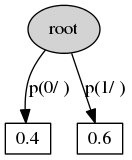
\includegraphics[scale=0.57]{img/sample_mixture/real_trie_.png}
	\centering
	\caption{ Реальное дерево }
	\label{ris:sample_mixture_real_trie}
	
\end{minipage}
\hfil \hfil%раздвигаем боксы по горизонтали
\begin{minipage}[b]{0.49 \textwidth}
	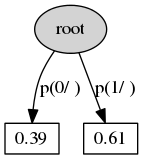
\includegraphics[scale=0.57]{img/sample_mixture/predicted_trie.png}
	\centering
	\caption{ Предсказанное дерево }
	\label{ris:sample_mixture_predicted_trie}
\end{minipage}
\end{figure}

\subsubsection{СММ}
Рисунок \ref{ris:sample_hmm1_real_trie} --- реальное дерево, множество распределений испусканий 
\\$B = \{\textit{Poisson}(1), \textit{Poisson}(8)\}$ 

Рисунок \ref{ris:sample_hmm1_predicted_trie} --- пример предсказанного дерева
\begin{tabbing}
% Эта строка только определяет ширину колонок.
MMMM \= MMMММM \= MMММMM \= MMММMM \= MМMМMM \kill
% Здесь начинается первая строка содержания таблицы.
\bf{}  \> {\bf $\textit{A}$} \> {\bf $\textit{lambda}$} \> {\bf $\textit{fdr}$} \> {\bf $\textit{fndr}$} \\ 
$\textit{MAE}$ \> $0.09$ \> $0.21$ \> $0.02$ \> $0.02$ \
\end{tabbing} 

Рисунок \ref{ris:sample_hmm1_log_likelihood} --- график логарифма правдоподобия по всем итерациям обучения. Грубо говоря, это карта обучения. На ней видно, как сначала алгоритм 6 итераций EM обучался на 16 контекстах, после чего дерево подстриглось до 2 контекстов. Следующему EM не удалось значимо увеличить правдоподобие модели, поэтому на третей итерации он закончил работу. Далее дерево не удалось еще раз подрезать, поэтому весь алгоритм закончил свою работу (это видно из отсутствия следующего бокса под график ЕM).
\begin{figure}[h!]\centering
\begin{minipage}[b]{0.49 \textwidth}
	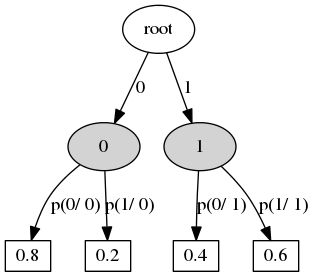
\includegraphics[scale=0.4]{img/sample_hmm1/real_trie_.png}
	\centering
	\caption{ Реальное дерево }
	\label{ris:sample_hmm1_real_trie}
\end{minipage}
\hfil \hfil%раздвигаем боксы по горизонтали
\begin{minipage}[b]{0.49 \textwidth}
	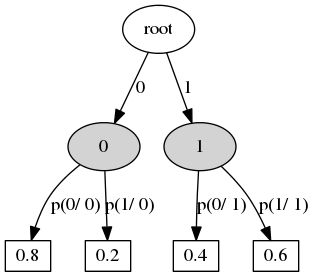
\includegraphics[scale=0.4]{img/sample_hmm1/predicted_trie.png}
	\centering
	\caption{ Предсказанное дерево }
	\label{ris:sample_hmm1_predicted_trie}
\end{minipage}
\begin{minipage}[b]{0.8 \textwidth}
	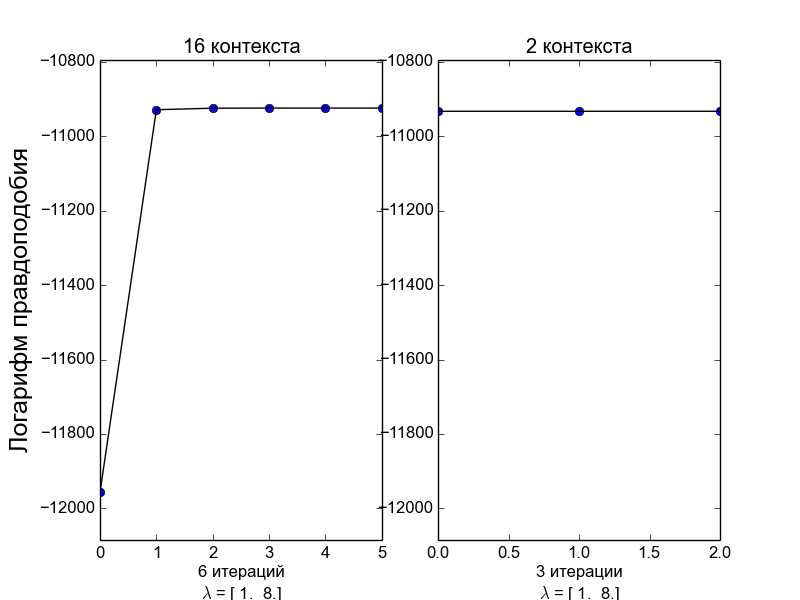
\includegraphics[scale=0.4]{img/sample_hmm1/plot_.png}
	\centering
	\caption{ Карта обучения }
	\label{ris:sample_hmm1_log_likelihood}
\end{minipage}
\end{figure}

\subsubsection{Более интересный случай, СММПП}
Рисунок \ref{ris:sample_real_trie} --- реальное дерево, множество распределений испусканий 
\\$B = \{\textit{Poisson}(3), \textit{Poisson}(15)\}$ 

Рисунок \ref{ris:sample_predicted_trie} --- пример предсказанного дерева
\begin{tabbing}
% Эта строка только определяет ширину колонок.
MMMM \= MMMММM \= MMММMM \= MMММMM \= MМMМMM \kill
% Здесь начинается первая строка содержания таблицы.
\bf{}  \> {\bf $\textit{A}$} \> {\bf $\textit{lambda}$} \> {\bf $\textit{fdr}$} \> {\bf $\textit{fndr}$}\\ 
$\textit{MAE}$ \> $0.11$ \> $0.20$ \> $0.02$ \> $0.02$ \
\end{tabbing}
Рисунок \ref{ris:sample_log_likelihood} --- график обучения.
\begin{figure}[h!]\centering
\begin{minipage}[b]{0.49 \textwidth}
	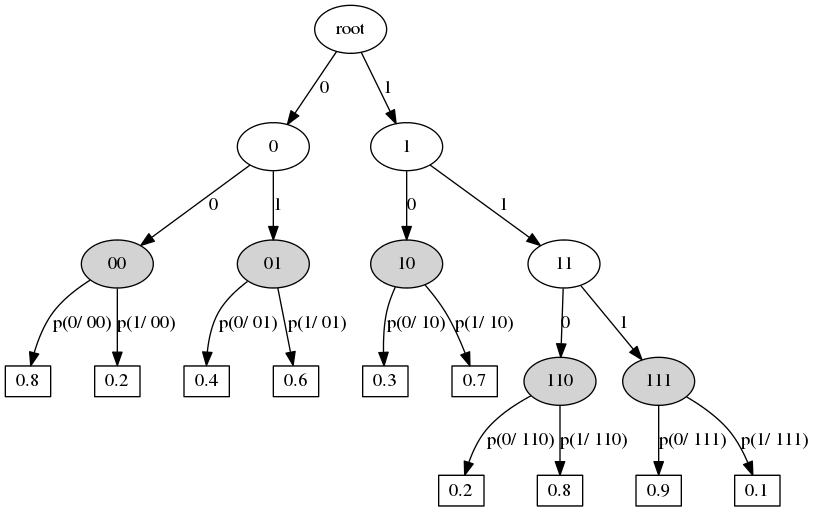
\includegraphics[scale=0.3]{img/sample/real_trie_.png}
	\centering
	\caption{ Реальное дерево }
	\label{ris:sample_real_trie}
	
\end{minipage}
\hfil \hfil%раздвигаем боксы по горизонтали
\begin{minipage}[b]{0.49 \textwidth}
	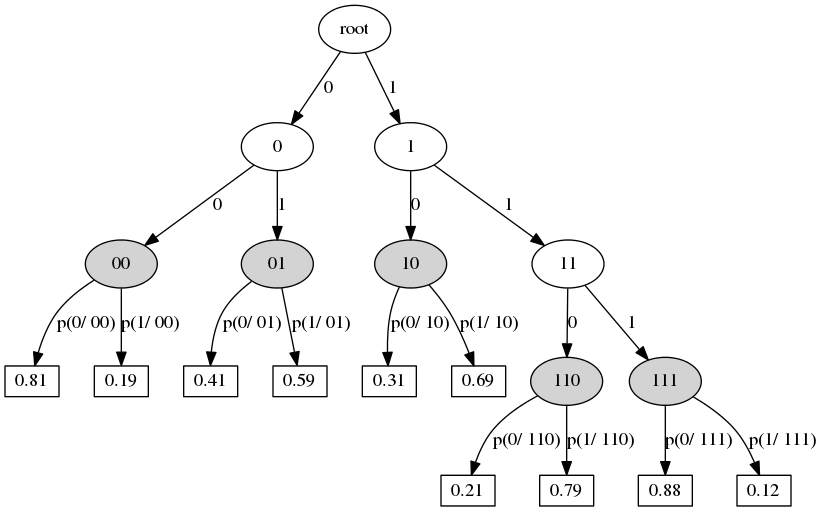
\includegraphics[scale=0.3]{img/sample/predicted_trie.png}
	\centering
	\caption{ Предсказанное дерево }
	\label{ris:sample_predicted_trie}
\end{minipage}
\begin{minipage}[b]{0.8 \textwidth}
	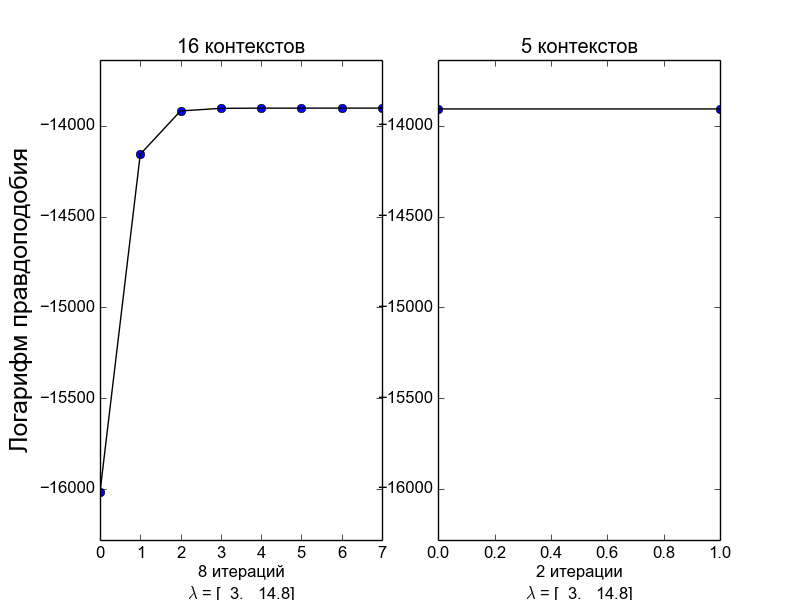
\includegraphics[scale=0.4]{img/sample/plot_.png}
	\centering
	\caption{ График обучения }
	\label{ris:sample_log_likelihood}
\end{minipage}
\end{figure}

\subsection{Применение к реальным данным}
Данные были взяты из проекта ENCODE (ENCyclopedia of DNA Elements).
В качестве исследуемого белка был выбран гистон H3 с ацетилированным лизином в 27-й позиции хвоста. Рассматриваемые клетки --- эмбриональные стволовые клетки человека \cite{ENCODE}.
Размер окна был выбран равный 200 п.н.

В качестве выборок были рассмотрены ненулевые участки вектора, полученного после деления результата эксперимента ChIP-seq на окна. 

Параметры обучения:\\
$m = 5$, $\epsilon_{\textit{prune}} = 0.04$, $\epsilon_{\textit{em}} = 0.05$
\begin{figure}[h!]\centering
\begin{minipage}[b]{0.49 \textwidth}
	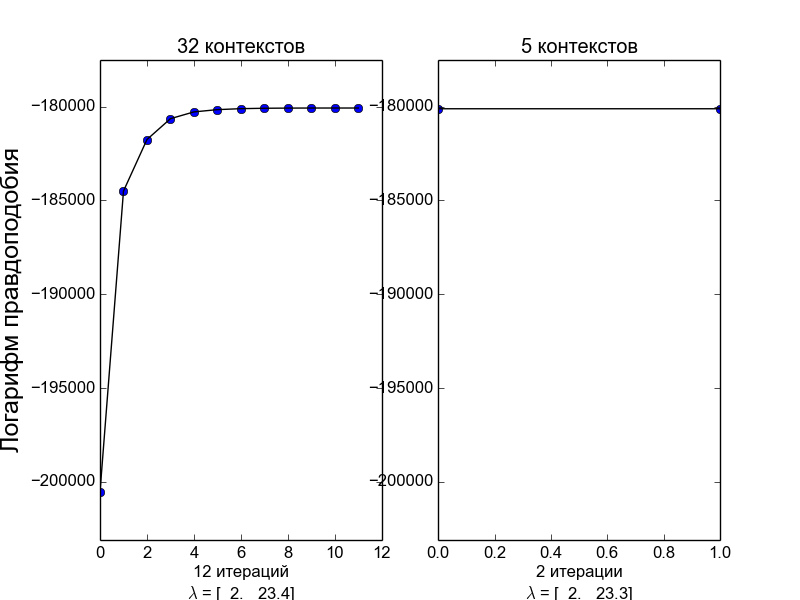
\includegraphics[scale=0.47]{img/real/plot_.png}
	\centering
	\caption{ График обучения }
	\label{ris:log_likelihood}
\end{minipage}
\hfill
\begin{minipage}[b]{0.32 \textwidth}
	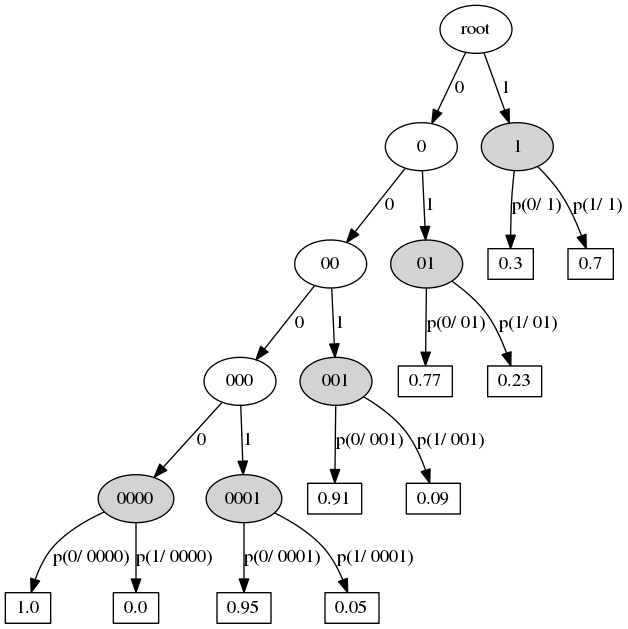
\includegraphics[scale=0.29]{img/real/predicted_trie.png}
	\centering
	\caption{ Контекстноe дерево }
	\label{ris:real_trie}
\end{minipage}
\end{figure}

Рисунок \ref{ris:log_likelihood} показывает, что сначала алгоритм 12 итераций EM обучался на 32 контекстах, потом подрезал дерево до 5 контекстов. После чего ни обучение, ни подрезание не дало результатов, поэтому, алгоритм закончил работу.

Рисунок \ref{ris:context_trie} показывает получившееся контекстное дерево.

Приведем таблицу сравнения для СММПП, СММ5 (СММ 5-го порядка, соответствует дереву, с которого мы начали обучения) и СММ (СММ 1-го порядка, именно его чаще всего используют для анализа данных ChIP-seq)
\begin{figure}[h!]\centering
\begin{minipage}[b]{0.32 \textwidth}
	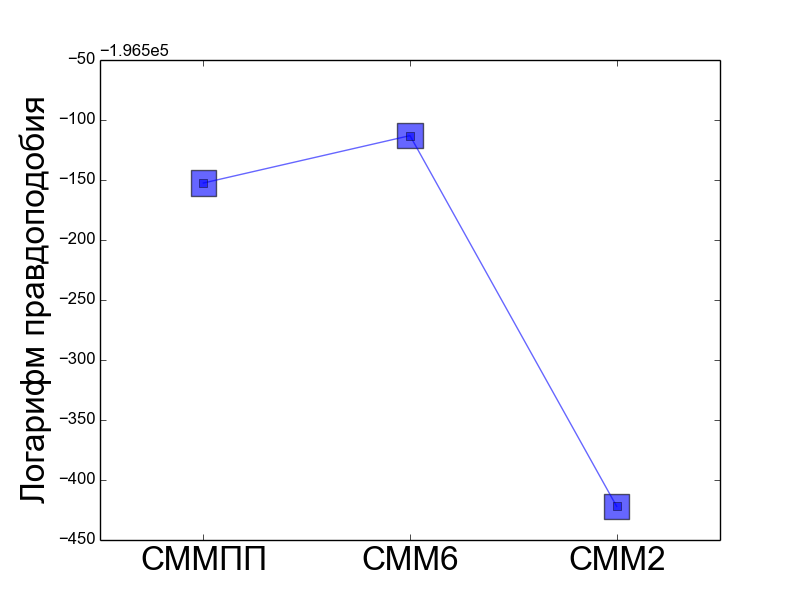
\includegraphics[scale=0.28]{img/real/log_p.png}
	\centering
	\caption{ Сравнение логарифма правдоподобия}
	\label{ris:real_comp_log_p}
\end{minipage}
\hfill
\begin{minipage}[b]{0.32 \textwidth}
	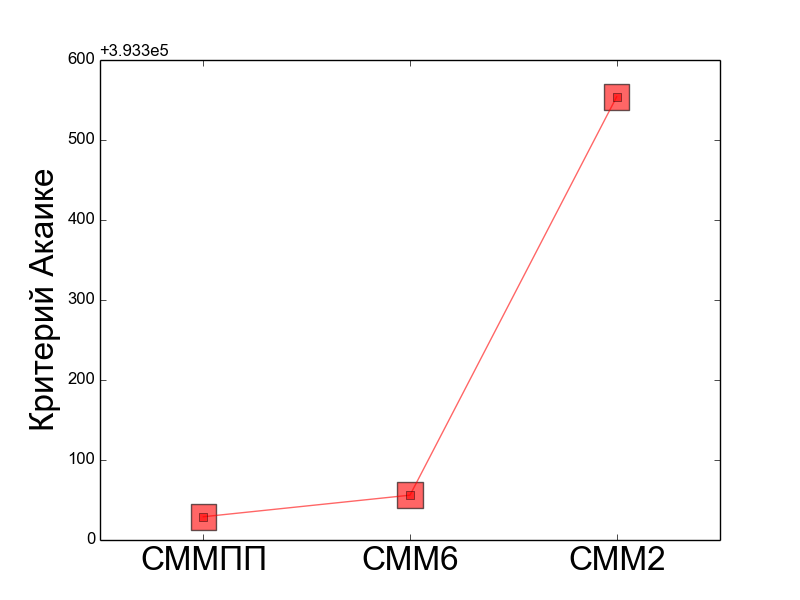
\includegraphics[scale=0.28]{img/real/aic.png}
	\centering
	\caption{ Сравнение критерия Акаике }
	\label{ris:real_comp_aic}
\end{minipage}
\hfill
\begin{minipage}[b]{0.32 \textwidth}
	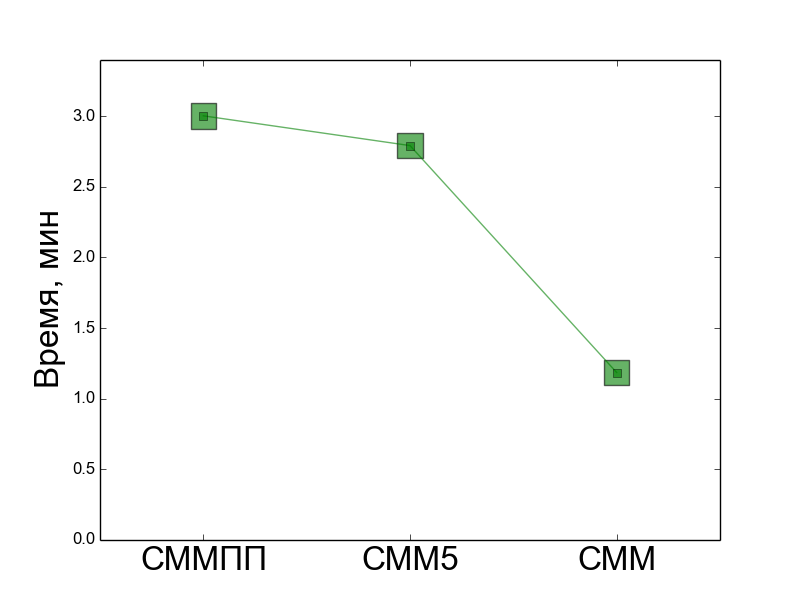
\includegraphics[scale=0.28]{img/real/time.png}
	\centering
	\caption{ Сравнение времени обучения }
	\label{ris:real_comp_time}
\end{minipage}
\end{figure}

На рисунке \ref{ris:real_comp_log_p} приведено сравнение правдоподобия моделей (в логарифмической шкале). Видно, что СММ5 лидирует. Однако СММПП ей не сильно уступает по сравнению с СММ.

Интересный результат показал критерий Акаике. Напомним, что данный критерий, чем меньше тем лучше. Сравнение его изображено на рисунке \ref{ris:real_comp_aic}.
Хотя СММ имеет гораздо меньшее количество параметров, чем СММПП, правдоподобие ее невилико, по этому по критерию Акаике она проигрывает. И наоборот, хотя СММ5 имеет лучшее среди этих трех моделей правдоподобие, оно имеет слишком много параметров, поэтому СММПП по критерию Акаике выигрывает и ее.

Рисунок \ref{ris:real_trie} показывает сравнение времени обучения. Тут СММПП дает похожий результат с СММ5, немного ей уступая. СММ, в силу того, что она имеет более простую структуру, обучается быстрее всех.


\section*{Заключение}
В ходе работы были решены поставленные задачи.
\begin{enumerate}
\item
Проанализированы существующие скрытые Марковские
модели переменного порядка, реализована подходящая под данные ChIP-seq модель.
\item
Проведен анализ эффективности работы модели на
синтетических данных, сравнение с более простыми
моделями (СММ первого порядка, пятого), 
\item
Осуществлено применение к
данным ChIP-seq
\end{enumerate}




\bibliographystyle{plain}
\bibliography{diploma.bib}
\end{document}
